\documentclass{VUMIFPSkursinis}

\usepackage{algorithmicx}
\usepackage{algorithm}
\usepackage{algpseudocode}
\usepackage{amsfonts}
\usepackage{amsmath}
\usepackage{bm}
\usepackage{caption}
\usepackage{color}
\usepackage{float}
\usepackage{graphicx}
\usepackage{listings}
\usepackage{subfig}
\usepackage{wrapfig}
\usepackage[backend=biber]{biblatex}
\usepackage[table,xcdraw]{xcolor}
\usepackage{booktabs}

\usepackage{enumitem}

\setitemize{noitemsep,topsep=0pt,parsep=0pt,partopsep=0pt}
\setenumerate{noitemsep,topsep=0pt,parsep=0pt,partopsep=0pt}

\setmainfont{Palemonas}

\university{Vilniaus universitetas}
\faculty{Matematikos ir informatikos fakultetas}
\department{Informatikos studijų programa}
\papertype{Kursinis darbas}
\title{Sinchroninių ir Asinchroninių integracijų mikroservisų architektūrose palyginimas ir analizė}
\titleineng{Synchronous and Asynchronous integrations in microservices architectures comparison and analysis}
\status{3 kurso 4 grupės studentas}
\author{Lukas Milašauskas}
\supervisor{Dr. Saulius Minkevičius}
\date{Vilnius – \the\year}

\bibliography{bibliografija}


\begin{document}


\maketitle
\cleardoublepage\pagenumbering{arabic}
\setcounter{page}{2}


\tableofcontents
\clearpage

\sectionnonum{Įvadas}

\subsectionnonum{Temos aktualumas}
Temos aktualumas
\subsectionnonum{Problema}
Problema
\subsectionnonum{Darbo tikslas}
Darbo tikslas
\subsectionnonum{Uždaviniai tikslui pasiekti}
\begin{enumerate}
	\item itemas
\end{enumerate}


\section{Kas yra mikroservisai}

\subsection{Monolitinės sistemos ir mikroservisų atsiradimas}
Pagal autorių Nicola Dragoni, Saverio Giallorenzo, Alberto Lluch Lafuente, Manuel Mazzara publikuotą straipsnį „Microservices: yesterday, today, and tomorrow“
\cite{Misc7} jau 1960-iais buvo susiduriama su problemomis susijusiomis su didžiulio masto PĮ kūrimu ir kaip tai projektuoti.
Buvo kuriama daug būdų kaip tai daryti, ir daug teorijų kaip tūrėtų atrodyti PĮ kodas, ir kaip projektuoti informacines sistemas.
Daug vėliau, apie 2000 metus, susiformavo sąvokos „Service-Oriented Computing“ (toliau SOC) ir „Service-Oriented Architecture” (toliau SOA), kurių idėja ir paradigmos buvo apie
tai, kad programa, arba kitaip pavadinus tarnyba, turėtų būti atsakingas už konkretaus resurso ar verslo logikos informaciją.
Šią tarnybą turi būti galima pasiekti su konkrečia technologija ir taip komunikuoti ir gauti informaciją. 
Taigi, remiantis jau ankščiau minėtu straipsniu „Microservices: yesterday, today, and tomorrow“ \cite{Mis7} iš SOC ir SOA kiek vėliau, susiformavo
mikroservisų idėja ir paradigmos. Pagal Martin Fowler ir James Lewis 2016-ais metais publikuotą straipsnį „Microservices“ \cite{Misc6}
šis terminas „mikroservisai“ buvo pirmą kartą diskutuotas 2011 metais, Venecijoje vykusiose PĮ kūrimo architektų
dirbtuvėse (angl. \textit{„workshop“}). Po metų, ta pati grupė architektų nusprendė, kad labiausiai tinkantis pavadinimas
šiam architektūriniam tipui yra mikroservisai (angl. \textit{„microservices“}). Po šiuo terminu slypi daug idėjų ir paradigmų,
tačiau pagrindinė mintis yra skaidymas didelės sistemos į mažas „granules“ ir mažas tarnybas.
Taip pat norint apibūdinti senas sistemas, kurios buvo nedalomos ir paleidžiamos vienu vykdomuoju paketu, atsirado terminas „monolitas“ (angl. \textit{„monolith“}).
Šis terminas ir buvo naudojamas Unix bendruomenės jau ilgą laiką iki mikroservisų susikūrimo.
Remiantis Eric Steven Raymon knyga „The Art of UNIX Programming“ \cite{Bk4}, kuri buvo išleista 2003 metais,
terminas „monolitas“ buvo naudojamas apibūdinti sistemoms, kurios yra per didelės. Taigi, šie du terminai
naudojami iki šiol apibūdinti informacinių sistemų architektūrinėms charakteristikoms.
\subsection{Mikroservisų pranašumai prieš monolitus}
Pagrindinius principus ir mikroservisų pranašumus detaliai išdėstė Sam Newman savo knygoje „Building Mircroservices: Designing Fine-Grained Systems“ \cite{Bk2}.
Šiame leidinyje autorius išgrynina keletą labai svarbių mikroservisų privalumų.
\subsubsection{Technologijų nevienalytiškumas (angl. \textit{„Technology Heterogeneity“})}
Kiekviena tarnyba turi atlikti skirtingas funkcijas ir turėti skirtingas atsakomybes. Norint pasiekti
geriausius rezultatus galima rinktis skirtingas technologijas, kurios būtų geriausiai pritaikytos konkrečiam uždaviniui spręsti.
Todėl mikroservisuose kiekvieną tarnybą galim projektuoti skirtingomis technologijomis, pavyzdžiui skirtingomis programavimo kalbomis.
\subsubsection{Atsparumas (angl. \textit{„Resilience“})}
Atsitikus problemai ir sugriuvus vienai sistemos komponentei, monolitinėje sistemoje tektų perkraudinėti arba taisyti visą sistemą.
Mikroservisų architektūroje stambių pasikeitimų būtų išvengta ir žlugtų tik vienos tarnybos veikimas. Tokiu atveju kitos tarnybos
apie tai nežinotų ir veiktų toliau, o norint ištaisyti problemą, užtektų sutaisyti ir perkrauti vieną tarnybą.
\subsubsection{Plečiamumas (angl. \textit{„Scaling“})}
Stambioje monolitinėje sistemoje visos plečiamumo ir efektyvumo problemos sprendžiamos kartu. Mikroservisų sistemoje
kiekvieną tokio tipo problemą sprendžiame atskirose tarnybose. Tokiu atveju tarnyboms, kurios reikalauja mažiau resursų
galima suteikti mažiau, o sunkesnioms ir mažiau efektyvioms tarnyboms išskirti daugiau.
Tačiau verta paminėti, kad mikroservisų sistemos plečiamumas ne visada yra geras, tai aprašyta
Omar Al-Debagy ir Peter Martinek straipsnyje „A Comparative Review of Microservices and Monolithic Architecture“ \cite{Misc3}
\subsubsection{Lengvas diegimas (angl. \textit{„Ease of Deployment“})}
Vystant PĮ dažnai susiduriama su diegimo problema. Su naujais funkcionalumais reikia iš naujo diegti naują PĮ versiją.
Monolitinėje sistemoje tenka iš naujo sudiegti visą sistemą, tačiau mikroservisų sistemoje galima sudiegti tik tas tarnybas, kurios yra susijusios
su pakeitimais.
\subsubsection{Organizacinis pasiskirstymas (angl. \textit{„Organizational Allignment“})}
Dažnai įmonėse prie informacinės sistemos dirba daug žmonių. Jie būna pasiskirstę komandomis ir turi skirtingas atsakomybes.
Mikroservisų sistemose galima išvengti komunikavimo incidentų ir kiekvienai komandai dirbti su skirtingomis tarnybomis.
Tokiu pavydžiu dirba stambi informacinių technologijų (toliau IT) įmonė „Netflix“.
\subsubsection{Kompozicija (angl. \textit{„Composability“})}
Įmonės dažnai susiduriama su problema, kai tas pats funkcionalumas reikalingas keliose informacinėse sistemose.
Mikroservisų architektūroje, kadangi sistema susideda iš mažų autonomiškų tarnybų, jas galima atskirti ir perpanaudoti
skirtingose sistemose, arba kitai sistemai suteikti prieigą tik prie konkrečių resursų, o ne visos sistemos.
\subsubsection{Optimizuotas pakeičiamumas (angl. \textit{„Optimizing for Replaceability“})}
Dirbant vidutinio dydžio arba didelėse imonėse dažnai susiduriama su problema, kai naudojama sena kodo bazė ir pasenusios technologijos.
Dažnai tokią sistemą reikia atnaujinti siekiant efektyvumo arba palaikymo paprastumo. Tokiu atveju, norint
atnaujinti bibliotekas arba technologijas, tenka iš naujo perprogramuoti dalį sistemos. Mikroservisų architektūros pagalba,
tai tampa žymiai papraščiau, kai užtenka perrašyti konkrečią tarnybą, neliečiant likusios informacinės sistemos.
\subsection{Monolitinių sistemų skaidymas į mikroservisus}
Paskutinį dešimtmetį tapo gan populiaru stambaus mąsto monolitus skaidyti į mikroservisus, tačiau tai nėra taip paprasta.
Visų pirma skaidant monolitą į atskiras tarnybas labai svarbu identifikuoti, kokios mažesnės tarnybos bus.
Tarnybų riboms apibrėžti panaudojau Micheal C. Feahters knygoje „Working Effectively with Legacy Code“ \cite{Bk5} apibrėžtą terminą
„siūlė“ (angl. \textit{„seam“}). Siūlė šiuo atveju yra kodo dalis, kuri yra izoliuota ir autonomiška.
Siūlės ir bus mūsų atskiri mikroservisai.
Autorė Susan J. Fowler savo knygoje „Production-Ready Microservices“ \cite{Bk1} aprašė patarimus ir žingsnius,
kaip reikėtų skaidyti monolitą į mikroservisus. Ji pamini, kad tai reikėtų daryti etapais:
\begin{enumerate}
	\item Monolitinę programą paleisti su tiek kopijų, kiek turėsime siūlių.
	\item Išskirstyti kvietimus į kopijas, pagal tai kokias siūles kopijos reprezentuoja.
	\item Išvalyti programų kopijas, paliekant tik siūlių funkcionalumą.
\end{enumerate}
Verta paminėti, kad po kiekvieno išvardinto žingsnio būtų atliekami regresiniai testavimai, kurie patikrintų
ar sistema veikia korektiškai.


\sectionnonum{Mikroservisų sistemos vidinių integracijų tipai}
Mikroservisų sistemos vidinių integracijų tipai


\sectionnonum{Sinchroninės (angl. “synchronous”) integracijos}

\subsectionnonum{Sinchroninių integracijų principas}
Sinchroninių integracijų principas
\subsectionnonum{Sinchroninių integracijų technologijų tipai}
Sinchroninių integracijų technologijų tipai


\sectionnonum{Asinchroninės (angl. “asynchronous”) integracijos}

\subsectionnonum{Asinchroninių integracijų principas}
Asinchroninių integracijų principas
\subsectionnonum{Asinchroninių integracijų technologijų tipai}
Asinchroninių integracijų technologijų tipai
\section{Skirtingų integracijų tipų privalumai ir trūkumai}


\subsection{Silpnas sujungimas ir stiprus sąryšis (angl. \textit{„Loose Coupling and High Cohesion“})}
Sinchronines ir asinchronines integracijas mikroservisuose galima palyginti pagal tai ar tai atitinka pagrindinius mikroservisų
kriterijus. Pagrindiniai principai pagal kuriuos galima teigti kad servisas yra tinkamai suprojektuotas yra \cite{Bk2}:

\begin{itemize}
  \item Silpnas sujungimas (angl. \textit{„Loose Coupling“}).Tai reiškia, kad kiekvienas servisas turėtų kuo labiau būti nepriklausomas. Jeigu yra daromas pakeitimas servisui, tai turėtų
  tik jam vienam ir būt atliekamas, nes vienas is pagrindinių mikroservisų privalumų yra galėjimas įdiegtį vieną servisą, nediegiant kitų.
  \item Stiprus sąryšis (anlg. \textit{„High Cohesion“}).Tai reiškia, kad kievkienas servisas tūretų savo logiką laikyti 
  pas save ir atlikti visus su savo atsakomybėmis susijusius procesus.
\end{itemize}

Šiuose dviejuose aspektuose ryškus asinchroninių integracijų pranašumas. Asinchroninių komunikacijų metu, servisai tiesiog siunčia pranešimus apie procesų pabaigą ir 
klausosi, kada juos pradėti. Sinchroninės komunikacijos reikalauja žinoti implementacijos detales ir kreiptis į kitus servisus, per klientus arba tiesiogiai.
Dažniausiai asinchroninės komunikacijos visoje sistemoje veikia vienodai.

\subsection{Efektyvumas}

Vienas pagrindinių skirtumų tarp sinchroninių ir asinchroninių integracijų yra blokavimas. Kaip jau minėta ankščiau
sinchroninės integracijos yra blokuojančios, priešingai nei asinchroninės. Kaip minima įmonės „Microsoft“
publikuotame darbe apie mikroservisus ir jų kūrimą su .NET technologija \cite{Misc1} vykdant ilgus ir daug resursų reikalaujančius procesus
pasitelkiant tokią technologiją kaip RESTful, dėl ilgo atsakymo laukimo galima patirti operacijos laiko pasibaigimus (angl. \textit{„timeouts“})
ir dėl to sėkmingai neužbaigti procesų.

Kitas asinchroninių integracijų privalumas yra lygiagretiškumas. Priešingai nei sinchroniniai komunikavimai,
pranešimus gali prenumeruoti ir vienu metu savo pareigybes vykdyti keli procesai, kas, žinoma, padidina sistemos
efektyvumą ir sutrumpina procesų veikimo laiką.

\subsection{Implementacijos kompleksiškumas}

Dar vienas labai svarbus faktorius renkantis tarp technologijų yra kompleksiškumas. Kuriant programinę įrangą kompleksiški reikalavimai
reiškia, kad atsiras daug vietos klaidoms. Klaidos labai stipriai didina gamybos kaštus ir sistemos vartotojų nepasitenkinimą.
Asinchroninės integracijos yra žymiai sudėtingesnės ir dažniausiai naudojami pranešimų brokeriai reikalauja papildomų 
implementacijos detalių, kad pavyktų sujungti servisą su brokeriu ir pavyktų klausytis arba publikuoti pranešimus.
Tokie darbai iš PĮ kūrėjų reikalauja aukštos kvalifikacijos, o tokių darbuotojų, kurie atitiktų reikalavimus,  įmonėms yra daug sunkiau surasti ir įdarbinti.
Kita vertus sinchroninės servisų kvietimai yra paprasti ir servisų applikacijų programavimo sąsajos būna išlaikomos primityvios ir trivelios.
Tas minima ir David S.Linthicum knygoje „Enterpise Application Integration“ \cite{Bk3}.

\subsection{Veiksmų istorija}

Kuriant dideles informacines sistemas, dažnai reikia atsižvelgti į įvykių registravimą. Dažnas reikalavimas didelėms sistemoms yra veiksmų istorija.
Tokiems uždaviniams spręsti geriausiai tinka asinchroninės užklausos, nes pasitelkus tokias technologijas kaip pranešimų brokeriai
žinutės ir įvykiai būna saugomi, ypač įvykiais paremtose (angl. \textit{„event-based“}) architektūrose.
Sinchroninių integracijų metų įvykių istorijos problemą reikia spręsti kitaip ir ji netampa tokia triveli.

\subsection{Įvykių sekos užtikrinimas}

Procesų vykdymai, kaip jau minėta studentų registracija, neretai reikalauja užtikrinimo, kad vienas procesas bus įvykdomas ankščiau už kitą.
Sinchroninės integracijos yra blokuojamos ir vykdomos paeiliui, todėl šios problemos nelieka, tačiau asinchroninis komunikavimas gali būti 
lygiagretinamas ir siekiant užtikrinti korektišką eiliškumą reikia įgyvendinti papildomos logiką. Dėl tokių atvejų, lygiagretūs procesai
tampa dar labiau komplikuoti. Tokiais atvejais asinchroninio komunikavimo metu servisai turi saugot proceso būseną ir užtikrinti veiksmų eiliškumą.

\subsection{Servisų perpanaudojimas}

Vienas iš mikroservisų architektūros privalumų yra išskaidytų servisų perpanaudojimas. Įmonės, kurios užsiima projektiniais darbais,
neretai siekia kurti tokią PĮ, kuria būtų galima pasiremti arba jos komponentes panaudoti ateities projektuose. Mikroservisai, kurie naudoja 
sinchronines integracijas būna mažiau surišti su domeno logika ir norint integruoti servisą kitoje informacinėje sistemoje
neprivaloma taip prisirišti prie technologijų. Tokie servisai įmonėms atneša daug naudos ir sutaupo kaštų ateityje.

\sectionnonum{Rezultatai ir išvados}

\subsectionnonum{Rezultatai}
Rezultatai
\subsectionnonum{išvados}
išvados

%% PAKEISTAS PAVADINIMAS Į 'Šaltiniai'
\printbibliography[heading=bibintoc, title=Šaltiniai]  % Šaltinių sąraše nurodoma panaudota
% literatūra, kitokie šaltiniai. Abėcėlės tvarka išdėstomi darbe panaudotų
% (cituotų, perfrazuotų ar bent paminėtų) mokslo leidinių, kitokių publikacijų
% bibliografiniai aprašai.  Šaltinių sąrašas spausdinamas iš naujo puslapio.
% Aprašai pateikiami netransliteruoti. Šaltinių sąraše negali būti tokių
% šaltinių, kurie nebuvo paminėti tekste.

% \sectionnonum{Sąvokų apibrėžimai}
Sąvokų apibrėžimai ir santrumpų sąrašas sudaromas tada, kai darbo tekste
vartojami specialūs paaiškinimo reikalaujantys terminai ir rečiau sutinkamos
santrumpos.


%\appendix  % Priedai
% Prieduose gali būti pateikiama pagalbinė, ypač darbo autoriaus savarankiškai
% parengta, medžiaga. Savarankiški priedai gali būti pateikiami ir
% kompaktiniame diske. Priedai taip pat numeruojami ir vadinami. Darbo tekstas
% su priedais susiejamas nuorodomis.

%\section{Neuroninio tinklo struktūra}
%\begin{figure}[H]
%    \centering
%    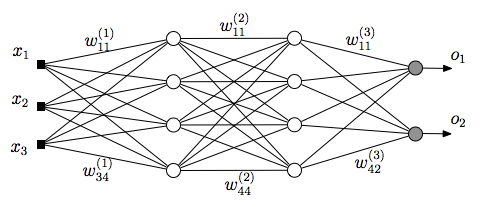
\includegraphics[scale=0.5]{img/MLP}
%    \caption{Paveikslėlio pavyzdys}
%    \label{img:mlp}
%\end{figure}

\end{document}
